% !TEX program = pdflatex
\documentclass[11pt]{article}

% ---------- Packages ----------
\usepackage[margin=1in]{geometry}
\usepackage{lmodern}
\usepackage[T1]{fontenc}
\usepackage[utf8]{inputenc}
\usepackage{microtype}
\usepackage{amsmath, amssymb, amsthm, mathtools}
\usepackage{bm}
\usepackage{enumitem}
\usepackage{booktabs}
\usepackage{graphicx}
\usepackage[dvipsnames]{xcolor}
\usepackage{hyperref}
\usepackage[capitalise,noabbrev]{cleveref}
\usepackage{algorithm}
\usepackage{algpseudocode}
\usepackage{placeins}

% ---------- Hyperref ----------
\hypersetup{
  colorlinks=true,
  linkcolor=MidnightBlue,
  citecolor=ForestGreen,
  urlcolor=RoyalBlue
}

% ---------- Theorem-like ----------
\theoremstyle{plain}
\newtheorem{theorem}{Theorem}
\newtheorem{proposition}{Proposition}
\newtheorem{lemma}{Lemma}
\theoremstyle{definition}
\newtheorem{definition}{Definition}
\newtheorem{remark}{Remark}

% ---------- Macros (notation kept minimal & consistent) ----------
\newcommand{\N}{\mathbb{N}}
\newcommand{\Z}{\mathbb{Z}}
\newcommand{\sig}[1]{\bm{\sigma}\!\left(#1\right)}           % σ(n) vector
\newcommand{\mass}{\mathrm{Mass}}                            % Mass(n)
\newcommand{\zcount}{\mathrm{ZeroCount}}                    % ZeroCount(n)
\newcommand{\tension}{\mathrm{T}}                           % T(n)
\newcommand{\curv}{\mathrm{C}}                              % C(n)
\newcommand{\phidet}{\Phi}                                  % Φ(n)
\newcommand{\Lone}[1]{\left\|#1\right\|_{1}}                % L1 norm
\newcommand{\spf}{\mathrm{SPF}}                             % smallest prime factor (if needed)
% --- Safe Greek in text/headings ---
% Use in text/headings as: ($\psi$-geometry), $\varphi$, $\Phi$

% Basis size (conceptual/for exposition)
\newcommand{\basis}{K}

% ---------- Canonical definitions (lock these) ----------
% Mass, ZeroCount, Tension
%   mass(n) = \|σ(n)\|_1; zero count = basis size - #used axes; T = mass * zero count.
% Curvature (centered 2nd-difference) and Phase Index (absolute-error normalized)
\newcommand{\MassDef}{\mass(n) := \Lone{\sig{n}}}
\newcommand{\ZeroDef}{\zcount(n) := \basis - \#\{\,i : e_i(n) > 0\,\}}
\newcommand{\TensDef}{\tension(n) := \mass(n)\cdot\zcount(n)}
\newcommand{\CurvDef}{\curv(n) := \Lone{\,\sig{n+1} - 2\,\sig{n} + \sig{n-1}\,}}
\newcommand{\PhiDef}{\phidet(n) := \dfrac{\big|\tension(n) - \curv(n)\big|}{\tension(n) + \curv(n)} \in [0,1]}

% ---------- Title ----------
\title{\Large Prime Emergence in Prime Exponent Space:\\
\large Rupture Dynamics and Canonical Structure}
\author{Kenneth Hilton}
\date{\today}

\begin{document}
\maketitle

\begin{abstract}
Primes appear irregular on the number line, yet in \emph{Prime Exponent Space} (PE-space) their emergence is structurally inevitable. Each integer $n$ is represented as a sparse vector of prime exponents, and along the successor map $n \mapsto n+1$ a new axis becomes necessary precisely at primes: the \emph{canonical carry}. We formalize this through smooth frontiers, carry economics, and an information balance $\psi(x)\sim x$, showing that the prime schedule is pointwise minimal.

On these foundations we introduce rupture dynamics via \emph{tension} and \emph{curvature}, consolidated in the normalized detector $\Phi(n)=\lvert T-C\rvert/(T+C)$. Empirically, $\Phi$ identifies pre-primes (frontier states with $n+1$ prime) with perfect recall across tested ranges, while precision pre-verifier follows the $1/\log n$ thinning of the Prime Number Theorem. Projected onto the golden-angle \emph{Saffron Spiral}, rupture spikes align into coherent ridgelines and exhibit intriguing legibility.

We extend this to a symbolic field view (potentials and forces), and deploy a recall-first pipeline (wheels + $\Phi$ + deterministic Miller–Rabin) that achieves recall $=1.0$ and precision $=1.0$ at scale, with $\Phi$ reducing verifier workload at fixed recall. Finally, we articulate a \emph{Universal Emergence Conjecture}: irreducible structures arise when redistribution fails. We present it explicitly as a conjecture to invite formal scrutiny and cross-disciplinary testing. All code and supporting documents are public for reproduction.
\end{abstract}


% ----------------------------------------------------------------
\section{Introduction and Motivation}

Prime numbers, long regarded as capricious and mysterious along the natural number line, can be reinterpreted as structurally inevitable when viewed through \emph{Prime Exponent Space} (PE-space). This representation encodes each integer $n \geq 2$ as a sparse vector of prime exponents, $\sigma(n) = (e_1,e_2,\dots)$, where $n=\prod p_i^{e_i}$, making the lattice of integers a geometric coordinate system rather than a mere list of values.

Traditional approaches to primes—sieves, analytic asymptotics, and primality tests—offer either exhaustive catalogues or global density laws, but do not illuminate the local structural mechanism of prime appearance. In PE-space, however, prime emergence is seen not as an accident but as a \emph{phase transition}: when existing prime axes can no longer redistribute symbolic mass, tension surpasses adaptability, and the system is forced to expand into a new dimension. This necessary dimension-creation event is the \emph{canonical carry}.

Our motivating axiom is simple yet potentially profound:

\begin{quote}
\paragraph{Universal Emergence Conjecture (informal).}
\emph{All irreducible structures appear when redistribution fails.}
(We state and discuss the conjecture formally in Sec.~10.)
\end{quote}

In arithmetic, this manifests as prime emergence. At $n \mapsto n+1$, if the composite lattice cannot accommodate the successor, the system ruptures and a new axis is born. In physical systems, we suggest the same principle governs fractures, phase changes, or ecological and cognitive thresholds. Thus, primes may provide the canonical, mathematically exact case of a universal phenomenon: emergence through redistribution failure.

This paper integrates multiple strands of our research:
\begin{itemize}
  \item \textbf{Phase dynamics.} Prime emergence as rupture events, quantified via tension, curvature, and the Phase Index.
  \item \textbf{Spiral geometry.} Projection of rupture dynamics onto the logarithmic golden-angle spiral (the \emph{Saffron Spiral}), revealing coherent ridgelines and resonances with galactic density waves.
  \item \textbf{Canonical carry calculus.} Formalization of smooth frontiers, carry economics, and information balance ($\psi(x) \sim x$) that show primes are the minimal and inevitable axes of arithmetic.
  \item \textbf{Field-theoretic lens.} Potentials and flows in symbolic space, where composites are elastic valleys and primes are singular peaks.
  \item \textbf{Empirical pipeline.} A recall-first $\Phi$ detector on PE-signatures, paired with wheel sieves and an orthogonal verifier, achieving perfect recall and precision at scale.
  \item \textbf{Interdisciplinary bridges.} Analogies to fracture mechanics, Kolmogorov complexity, edge-of-chaos dynamics, Gödel incompleteness, and Chaitin irreducibility.
\end{itemize}

Our goal is not merely to propose a new prime-detection algorithm, but to position prime emergence as a structural inevitability within a universal theory of irreducibility. By assembling the fragments—structural metrics, geometric projections, canonical carry, symbolic field theory, and empirical validation—we aim to provide the mathematical community with a coherent, reproducible, and extensible framework. This is both a synthesis of our prior works and an invitation for others to carry the theory further.

\paragraph{Scope and Claims (at a glance).}
\begin{itemize}[leftmargin=1.5em]
  \item \textbf{Proved:} canonical carry/frontier minimality; information balance $\psi(x)\sim x$; formal link of primes to exits from $p_k$-smooth semigroups.
  \item \textbf{Empirical:} $\Phi$ concentrates at pre-primes (recall $=1.0$ on tested ranges); pre-verifier precision tracks $1/\log n$; $\Phi$ reduces verifier workload at fixed recall.
  \item \textbf{Conjectural:} Universal Emergence Conjecture; Saffron Spiral exposes prime emergent structure; field-theoretic analogies beyond arithmetic.
\end{itemize}

% ----------------------------------------------------------------
% ----------------------------------------------------------------
\section{Prime Exponent Space: Definitions and Conceptual Framework}

The foundation of our approach is \emph{Prime Exponent Space} (PE-space), a coordinate system on $\N_{\geq 1}$ induced by unique factorization. Every integer $n \geq 2$ can be expressed as
\[
n = \prod_{i=1}^k p_i^{\,e_i} 
\quad \Longleftrightarrow \quad
\sigma(n) = (e_1, e_2, \ldots, e_k, 0, 0, \ldots),
\]
where $p_1=2, p_2=3, \dots$ are the primes in order, and only finitely many exponents $e_i$ are nonzero. Thus $\sigma(n)$ is a sparse, finite-support vector encoding $n$ in multiplicative coordinates. This mapping is bijective by the Fundamental Theorem of Arithmetic.

\subsection{Geometric Properties}
\begin{itemize}
  \item \textbf{Multiplication and Division.} In PE-space, multiplication corresponds to vector addition and division to subtraction:
  \[
  \sigma(a \cdot b) = \sigma(a) + \sigma(b), 
  \qquad 
  \sigma\!\left(\frac{a}{b}\right) = \sigma(a) - \sigma(b).
  \]
  \item \textbf{GCD and LCM.} Greatest common divisors and least common multiples reduce to pointwise min and max operations on the coordinates:
  \[
  \gcd(a,b) = \prod_i p_i^{\min(e_i^a,e_i^b)},
  \qquad
  \mathrm{lcm}(a,b) = \prod_i p_i^{\max(e_i^a,e_i^b)}.
  \]
  \item \textbf{Dimensional Expansion.} Composites occupy the expressive capacity of existing axes; primes mark the first use of a new axis. Thus each prime introduces a new dimension into PE-space.
\end{itemize}

\subsection{Smooth Frontiers and Pre-Primes}
For $k \geq 1$, define the $p_k$-smooth semigroup
\[
S_k = \Bigl\{ \prod_{i=1}^k p_i^{\,e_i} : e_i \in \N_0 \Bigr\},
\]
the set of integers using only the first $k$ primes.  
A \emph{pre-prime at level $k$} is an $n \in S_k$ such that $n+1 \notin S_k$.  
The \emph{emergence threshold} theorem states:
\[
p_{k+1} = \min(\N_{\geq 2} \setminus S_k), 
\qquad p_{k+1}-1 \in S_k,
\]
so that $p_{k+1}-1 \mapsto p_{k+1}$ is the canonical moment where a new axis $e_{k+1}$ is forced.

\subsection{Conceptual Benefits}
Representing integers in PE-space provides:
\begin{enumerate}
  \item \textbf{Structural clarity.} The multidimensionality of arithmetic is exposed explicitly; primes are seen as axis-creation events, not as random anomalies.
  \item \textbf{Framework for prediction.} Local metrics—mass, tension, curvature—can be defined directly on $\sigma(n)$, providing predictive power for identifying rupture points where redistribution fails.
  \item \textbf{Universality.} The coordinate perspective situates arithmetic alongside analogous coordinate systems in physics, complexity theory, and information theory, enabling interdisciplinary bridges.
\end{enumerate}

\subsection{Interpretive Remark}
While base-$B$ positional systems generate constant-rate digit carries ($\E[\#\text{carries}] = 1/(B-1)$), PE-space exhibits \emph{canonical carries} only at primes, with frequency $\sim 1/\log n$. This contrast highlights that primes are not accidents of factorization but are structurally enforced by the arithmetic lattice itself.

% ----------------------------------------------------------------
% ----------------------------------------------------------------
\section{Structural Metrics and the Normalized Detector}

Having established Prime Exponent Space (PE-space) as the structural lattice for the integers, we now define the quantitative metrics that allow us to detect rupture points—states immediately preceding prime emergence. These metrics derive from the geometry of $\sigma(n)$ and its neighbors.

\subsection{Symbolic Mass and Zero Count}
\begin{itemize}
  \item \textbf{Mass.} The symbolic mass of $n$ is the $L^1$ norm of its PE-vector:
  \[
    \mass(n) = \|\sigma(n)\|_1 = \sum_i e_i(n).
  \]
  It measures the total multiplicative complexity of $n$.

  \item \textbf{Zero Count.} The number of unused axes in the working basis of primes up to some $p_K$:
  \[
    \zcount(n) = K - \#\{\,i : e_i(n) > 0\,\}.
  \]
  Sparse factorizations (few prime factors) yield high zero count.
\end{itemize}

\subsection{Tension}
We define \emph{tension} as the product of mass and zero count:
\[
\tension(n) = \mass(n) \cdot \zcount(n).
\]
Tension quantifies rigidity: high $\tension(n)$ indicates that the number’s structure is saturated and near the edge of redistribution capacity.

\subsection{Curvature (Centered Stencil)}
Adaptability is measured by curvature, defined as the discrete second difference over the centered stencil $(n-1,n,n+1)$:
\[
\curv(n) = \Bigl\|\, \sigma(n+1) - 2\sigma(n) + \sigma(n-1) \,\Bigr\|_1.
\]
This captures local bending of the trajectory through PE-space. Low curvature signals brittleness, often immediately before prime emergence.

\subsection{Normalized Detector $\Phi$}
We combine rigidity and adaptability into a single contrastive metric. The \emph{normalized $\Phi$ detector} is:
\[
\phidet(n) = \frac{|\tension(n) - \curv(n)|}{\tension(n) + \curv(n)} \;\in [0,1].
\]
This \emph{absolute-error form}, adopted in our codebase, ensures scale invariance and sharp localization of frontier states.  

Empirically, $\phidet(n)$ approaches 1 at \emph{pre-primes}—those $n$ such that $n+1$ is prime—reflecting maximal imbalance between high tension and minimal curvature.

\paragraph{Why $\boldsymbol{\Phi}$ concentrates at frontier points.}
A convenient identity is
\[
\phidet(n) \;=\; 1 \;-\; \frac{2 \times \min\{\tension(n),\,\curv(n)\}}{\tension(n)+\curv(n)}\,.
\]
Thus $\phidet(n)\to 1$ whenever $\tension(n)\gg \curv(n)$. With a fixed working basis up to the scan cap, $\tension$ scales with the basis size (load $\times$ slack), whereas $\curv$ is a local $L^1$ second difference over $(n\!-\!1,n,n\!+\!1)$. Empirically this contrast is largest at frontier states (pre-primes), giving high recall. We do not claim a theorem here; we provide mechanism and data.

\subsection{Interpretation}
\begin{itemize}
  \item $\tension(n)$ grows with both accumulated multiplicative complexity and sparsity of factorization.
  \item $\curv(n)$ collapses when redistribution pathways flatten.
  \item $\phidet(n)$ highlights rupture: composites with elastic redistribution yield $\Phi$ well below 1, while frontier states push $\Phi$ toward unity.
\end{itemize}

Thus, $\phidet$ serves as a recall-first detector: it identifies all true rupture points, with false positives interpretable as \emph{elastic near-primes}—numbers mimicking rupture but resolving their strain without new axes.  
Later sections detail how wheels, guards, and orthogonal verification collapse these false positives while preserving recall.

% ----------------------------------------------------------------
% ----------------------------------------------------------------
\section{Canonical Carry, Smooth Frontiers, and Minimality}

The preceding section introduced local metrics of rigidity and adaptability in PE-space. We now place these in the broader arithmetic framework of \emph{canonical carries}: dimension-increase events that occur exactly at primes.

\subsection{Smooth Frontiers and Emergence Threshold}
For each $k \geq 1$, define the $p_k$-smooth semigroup
\[
S_k = \Bigl\{ \prod_{i=1}^k p_i^{e_i} : e_i \in \N_0 \Bigr\}.
\]
These are the integers whose prime factors are bounded by $p_k$.  

\begin{definition}[Pre-prime at level $k$]
An integer $n \in S_k$ is a \emph{pre-prime at level $k$} if $n+1 \notin S_k$.
\end{definition}

\begin{proposition}[Emergence threshold]
Let $S_k:=\{\prod_{i=1}^k p_i^{e_i}: e_i\in\N_0\}$ be the $p_k$-smooth semigroup. Then
\[
p_{k+1}=\min(\N_{\ge 2}\setminus S_k)\quad\text{and}\quad p_{k+1}-1\in S_k.
\]
\end{proposition}
\begin{proof}[Proof (immediate)]
By definition, $p_{k+1}$ is the smallest integer with a prime factor $>p_k$, hence it is the minimal element outside $S_k$; its predecessor has all factors $\le p_k$.
\end{proof}


\begin{remark}[Canonical carry]
The transition $p_{k+1}-1 \to p_{k+1}$ is a basis-free event. No matter the representation, unique factorization enforces this new axis. This successor step is the \emph{canonical carry}.
\end{remark}

\subsection{Carry Economics: Radix vs. Canonical}
Positional systems in base $B$ exhibit constant-rate carries: the expected number of digit carries per increment is
\[
\E[\#\text{carries on } n \mapsto n+1] = \frac{1}{B-1}.
\]
In contrast, canonical carries in PE-space occur exactly at primes, with frequency
\[
\Pr(n+1 \text{ is prime}) \sim \frac{1}{\log n} \quad (n \to \infty),
\]
as given by the Prime Number Theorem.  

\textbf{Interpretation.}  
Radix carries are frequent renormalizations along a collapsed axis; canonical carries are sparse but profound, introducing entirely new dimensions. Arithmetic thus economizes its structural innovation: new axes appear rarely but necessarily.

\subsection{Information Balance ($\psi$-geometry)}
Each prime event $p$ introduces payload $\log p$. The Chebyshev function
\[
\psi(x) = \sum_{p^a \leq x} \log p
\]
satisfies $\psi(x) \sim x$.  

\begin{proposition}[Balanced flux]
Sparse events (primes) multiplied by their payload (logarithmic weight) yield a linear information flux:
\[
\psi(x) \sim x.
\]
Thus, the canonical prime basis introduces axes rarely but meaningfully; their cumulative contribution balances perfectly against the growth of the integers.
\end{proposition}

\subsection{Minimality of Canonical Carries}
\begin{proposition}[Pointwise minimality]
Let $\mathcal{C}$ be the class of multiplicative coordinate systems on $\N_{\geq 1}$ that are injective and respect factorization.  
Then along $n \mapsto n+1$, the set of dimension-increase indices for any system in $\mathcal{C}$ must include the primes. Consequently, the mean event rate is $\asymp 1/\log n$.
\end{proposition}

\paragraph{Consequence.}
Primes form the \emph{minimal schedule} of dimension-increase events in arithmetic. Any consistent coordinate system is forced to expand precisely at the primes. This minimality anchors primes not as curiosities, but as the irreducible backbone of number structure.


% ----------------------------------------------------------------
% ----------------------------------------------------------------
\section{Rupture Dynamics: Pre-Primes as Inflection Points}

Prime emergence can now be interpreted as a rupture phenomenon: a structural phase transition in which accumulated symbolic tension overwhelms curvature and forces the system into a new axis. The states immediately preceding primes—\emph{pre-primes}—are the arithmetic equivalent of fault lines in materials science or edge-of-chaos states in complexity theory.

\subsection{Pre-Primes as Critical States}
We define a pre-prime $n$ as an integer where:
\[
\tension(n) \;\text{ is near maximal}, \qquad \curv(n) \;\text{ is near minimal},
\]
so that
\[
\phidet(n) \approx 1.
\]
These conditions capture the critical balance: maximum symbolic stress, minimum adaptability. Crossing this boundary forces the successor $m=n+1$ into primality.

\subsection{Elastic vs. Rupture Outcomes}
Empirically, not all high-$\Phi$ candidates yield primes. False positives occur when a number exhibits high tension and low curvature but nonetheless absorbs strain through redistributive elasticity.  
\begin{itemize}
  \item \textbf{True rupture:} $n$ is a pre-prime, $n+1$ is prime.  
  \item \textbf{Elastic collapse:} $n$ mimics rupture conditions but $n+1$ factors; symbolic strain is absorbed without new dimension.
\end{itemize}
These elastic collapses are structurally meaningful—they are the near-primes, “almost ruptures,” analogous to metastable states in physics or unexpressed insights in cognition.

\subsection{Phase Transition Analogy}
This rupture mechanism parallels phase transitions:
\begin{itemize}
  \item In \textbf{physics}, stress beyond elasticity yields fractures and new surfaces; in PE-space, primes expand the dimensional lattice.
  \item In \textbf{complexity theory}, edge-of-chaos states mark maximal entropy and minimal adaptability, preceding qualitative shifts. Pre-primes occupy the same role in arithmetic.
  \item In \textbf{information theory}, pre-primes correspond to maximal Kolmogorov complexity (incompressibility). Prime emergence is the dimensional innovation that restores compressibility.
\end{itemize}

\subsection{Fault-Line Interpretation}
By scanning integers with $\Phi$, one traces ridgelines of stress through number space. These are arithmetic \emph{fault lines}, continuous bands of near-critical states culminating in rupture at primes.  
Visualization on the Saffron Spiral shows these ridgelines coalescing into coherent arms, reinforcing the view that prime emergence is not random but structured.

\subsection{Summary}
\begin{quote}
\emph{Pre-primes are the numeric inflection points where symbolic stress saturates and adaptability collapses.}  
Some resolve elastically, others rupture irreversibly into primes.  
This duality reframes prime prediction: not as an oracle, but as a phase-transition calculus of tension and collapse.
\end{quote}
 

% ----------------------------------------------------------------
% ----------------------------------------------------------------
\section{The Saffron Spiral: Geometry and Coherent Ridgelines}

While $\Phi(n)$ identifies rupture precursors along the one-dimensional number line, the underlying structure becomes clearer when projected into two dimensions. We employ a logarithmic spiral parameterized by the golden ratio, which distributes points evenly and reveals coherent ridgelines of pre-primes.

\subsection{Spiral Projection}
Each integer $n$ is mapped to polar coordinates
\[
r = \log n, 
\qquad \theta = \varphi n \pmod{2\pi}, 
\qquad \varphi = \frac{1+\sqrt{5}}{2},
\]
where $\varphi$ is the golden ratio. This construction, termed the \emph{Saffron Spiral}, resembles phyllotaxis patterns in botany and density waves in spiral galaxies.

\subsection{Coherent Ridgelines}
When plotted, rupture spikes do not scatter randomly. Instead, they align into continuous \emph{ridgelines}, spiral arms of concentrated pre-prime activity. These ridgelines trace arithmetic “fault lines” through PE-space, visually exposing the ordered geometry behind prime emergence.  

At larger scales, empirical studies confirm that ridgelines persist even as density falls, with precision decay following the $1/\log n$ form predicted by the Prime Number Theorem.

This resonance is not an arithmetic identity but a \emph{structural legibility property}: the irrational winding angle and Fibonacci shells together maximize coherence, much as in natural growth and galactic structure.

\subsection{Visualizations}
\noindent\textbf{Reproducibility:} The figure (below) was generated with the following command line:

\begin{verbatim}
python saffron_synthesis_master_v3_monolith.py --nmin 3 --nmax 10003 \
--threshold 0.17 --preprime-wheel 30 --prime-wheel 210 --peak-radius 1 \
--gate-c on --png saffron_spiral_3_10003.png
\end{verbatim}

\begin{figure}[h!]
  %\centering
  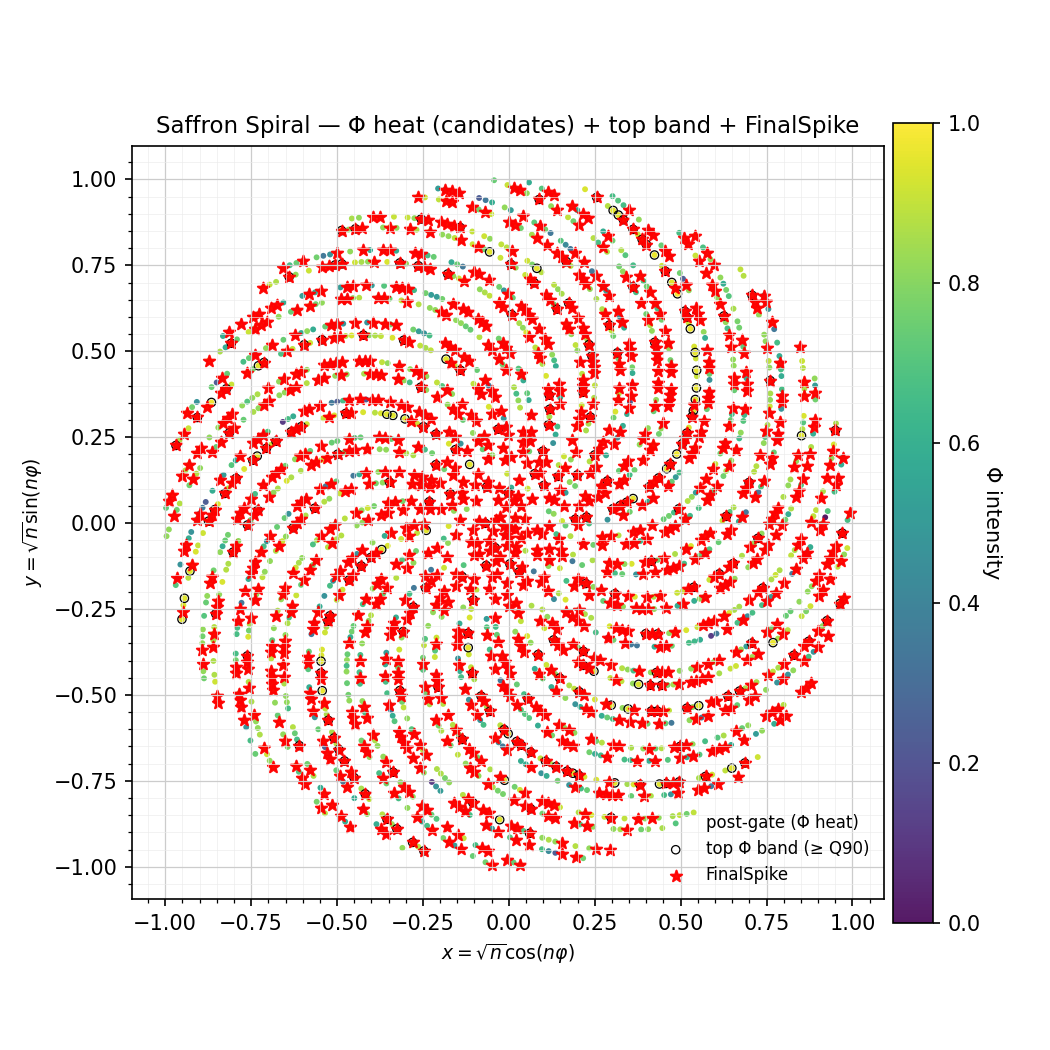
\includegraphics[width=0.9\linewidth]{saffron_spiral_3_10003.png}
  \caption{Heat-mapped Saffron Spiral for the window $n \in [3,10003]$:  
           $\Phi$ heat colored candidates with black rim for $\Phi$ > $\tau$, and verified pre-primes (red stars).}
  \label{fig:saffron-spiral-heatmap}
\end{figure}
\FloatBarrier

\noindent\textbf{Reproducibility:} The figure (below) was generated with the following command line:

\begin{verbatim}
python saffron_synthesis_master_v3_monolith.py --nmin 10000000 --nmax 10010030 \
--threshold 0.9985 --preprime-wheel 210 --prime-wheel 30030 --peak-radius 1 \
--gate-c on --png spiral_10M_10.1M.png
\end{verbatim}

\begin{figure}[h!]
  %\centering
  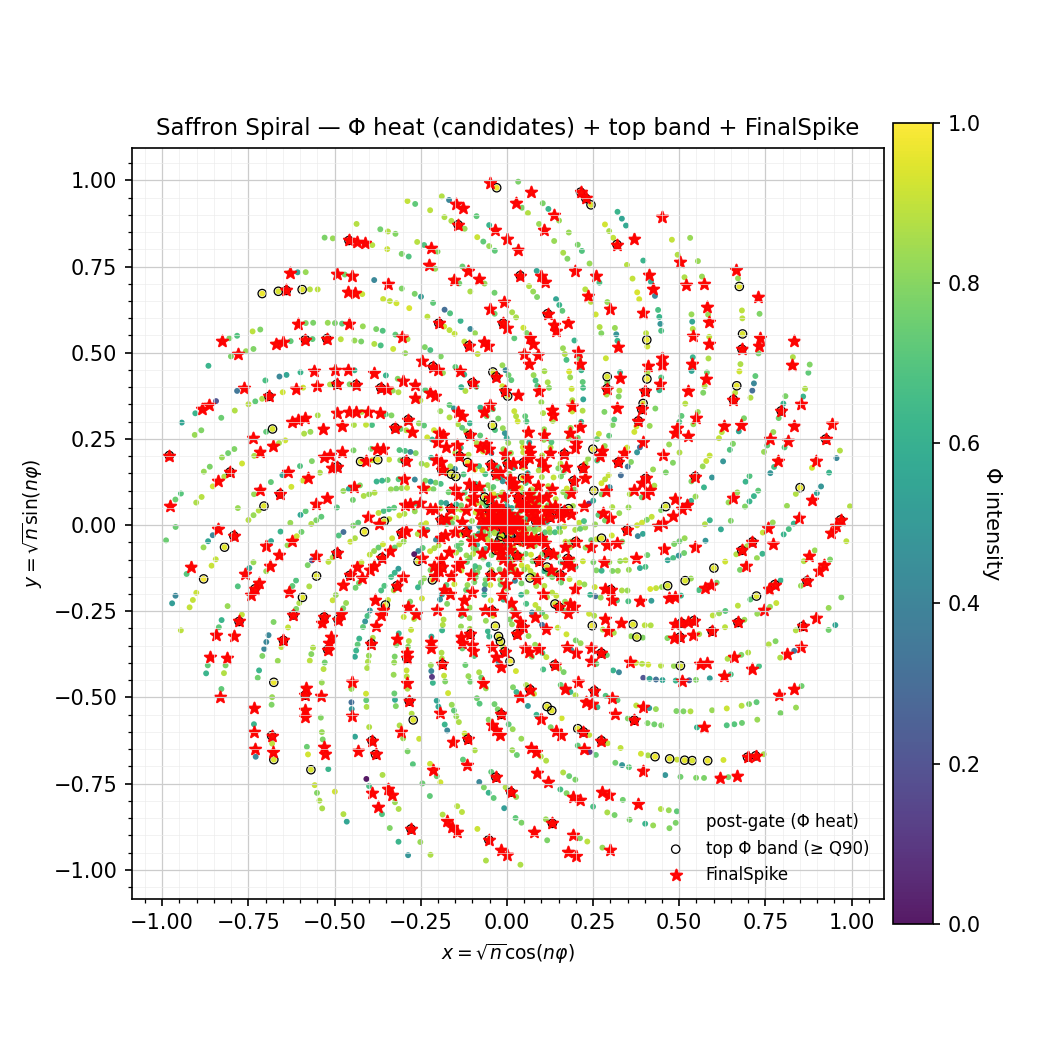
\includegraphics[width=0.9\linewidth]{spiral_10M_10.1M.png}
  \caption{Heat-mapped Saffron Spiral for the window $n \in [10000000,10010030]$:  
           $\Phi$ heat colored candidates with black rim for $\Phi$ > $\tau$, and verified pre-primes (red stars).}
  \label{fig:saffron-spiral-heatmap}
\end{figure}
\FloatBarrier

\subsection{Interpretation}
The spiral projection transforms local rupture spikes exposing global coherence:
\begin{quote}
\emph{The Saffron Spiral suggests prime emergence is not a random scatter but a resonance phenomenon.  
Rupture events trace ridgelines in number space, echoing the same mathematics that organizes leaves, shells, and galaxies.}
\end{quote}

% ----------------------------------------------------------------
% ----------------------------------------------------------------
\section{Symbolic Field View: Potentials, Forces, and Flows}

Beyond discrete metrics, prime emergence may be understood dynamically by treating PE-space as a symbolic field. In this interpretation, composites occupy elastic valleys of adaptability, while primes appear as singular peaks—points where redistribution collapses.

\subsection{Symbolic Potential}
We define a potential landscape encoding rupture susceptibility:
\[
\Phi_{\text{pot}}(n) = -\log\!\bigl(\phidet(n)\bigr) + \lambda \cdot \curv(n),
\]
where $\lambda$ is a smoothing parameter.  
\begin{itemize}
  \item The $-\log\!\phidet(n)$ term amplifies rupture instability: higher $\phidet$ signals brittle, near-prime states.  
  \item The curvature term stabilizes adaptable composites, smoothing the potential.  
\end{itemize}

\subsection{Symbolic Force}
Analogous to physics, force is the gradient of potential:
\[
F(n) = -\Delta \Phi_{\text{pot}}(n) = -\bigl(\Phi_{\text{pot}}(n+1) - \Phi_{\text{pot}}(n)\bigr).
\]
This discrete symbolic force directs trajectories toward rupture peaks or away into elastic basins.

\subsection{Flow Dynamics}
We model symbolic flow as a discrete dynamical system:
\[
n_{t+1} = n_t + \alpha \cdot F(n_t),
\]
where $\alpha$ sets the traversal scale.  
\begin{itemize}
  \item Trajectories converge toward prime emergence zones (singularities).  
  \item Trajectories diverge or oscillate in elastic composite regions.  
\end{itemize}
This reframes arithmetic as a symbolic flow field, with prime numbers as invariant attractors.

\subsection{Spiral Attractors and Interference}
When trajectories are projected back onto the Saffron Spiral:
\begin{itemize}
  \item \emph{Attractor basins} emerge: numeric regions converging on spiral ridgelines, aligning with prime loci.  
  \item \emph{Interference bands} appear: oscillatory patterns distinguishing highly composite zones from brittle rupture zones.  
\end{itemize}
These features resemble certain physical systems, where local perturbations reinforce long-range spiral order.

\subsection{Interpretation}
The field view complements the rupture model:
\begin{itemize}
  \item Tension $\mapsto$ symbolic energy.  
  \item Curvature $\mapsto$ elasticity of structure.  
  \item $\phidet$ peaks $\mapsto$ singular rupture points (primes).  
\end{itemize}
False positives become interpretable as elastic valleys—zones capable of absorbing strain without new axes.  

\begin{quote}
\emph{What begins as arithmetic metrics becomes a symbolic physics:  
a redistribution field, strained until rupture creates the irreducible.}
\end{quote}

% ----------------------------------------------------------------
% ----------------------------------------------------------------
\section{Empirical Pipeline: Gates, Thresholding, Orthogonal Verifier}

The structural metrics and field interpretation yield a high-recall rupture detector. To deploy this effectively at scale, we integrate them into a multi-stage pipeline that balances recall and precision, ensuring all true primes are identified while false positives are systematically eliminated.

\subsection{Gate A/B: Wheel Sieves}
\begin{itemize}
  \item \textbf{Gate A (on $n$).} Pre-prime wheel filter: exclude candidates divisible by small primes.  
  \item \textbf{Gate B (on $m=n+1$).} Prime wheel filter: eliminate successors $m$ with trivial factors.  
\end{itemize}
Practical implementations scale $(A,B)$ with the search range. For example, $(210,30030)$ balances efficiency and density at magnitudes beyond $10^7$.  

When Gate B includes the prime 2, Gate A is disabled to avoid parity conflicts (a refinement confirmed in code and practice).

\subsection{Phase Thresholding}
For each candidate $n$ passing wheels, compute
\[
\phidet(n) = \frac{|\tension(n) - \curv(n)|}{\tension(n) + \curv(n)}.
\]
Candidates with $\Phi(n) > \tau$ are flagged. The effective choice of $\tau$ depends on the 
scale of the scanning window: for small windows ($n \leq 10^{4}$), normalized $\Phi$ values 
sit in a lower numeric range, so recall-first operation typically uses $\tau \approx 0.15$--$0.20$; 
for large windows ($n \geq 10^{5}$), $\Phi$ values concentrate near unity, and recall-first 
operation uses $\tau \approx 0.998$--$0.999$. In all cases, $\tau$ is tuned to lie in the 
extreme upper tail of the observed $\Phi$ distribution (e.g., $\geq 99.8^{\mathrm{th}}$ percentile), 
ensuring perfect recall while tolerating a controlled set of false positives for later elimination 
by Gate~C.

\subsection{Peak Guard}
Optionally, retain only local maxima of $\phidet$ within a small neighborhood (radius $r \in \{0,1\}$). This suppresses redundant spikes while preserving recall.

\subsection{Gate C: Orthogonal Verifier}
The successor $m=n+1$ is subjected to a deterministic Miller–Rabin primality test with fixed bases (e.g., $\{2,3,5,7,11,13,17\}$).  
\begin{itemize}
  \item This verification is factor-free: no factorization of $m$ is performed.  
  \item Orthogonality arises because $\Phi$ depends only on $\sigma(n)$, while Gate C depends only on the multiplicative group $(\mathbb{Z}/m\mathbb{Z})^\times$.  
  \item Their error modes are independent; together, they yield precision $=1.0$ and recall $=1.0$ across tested ranges.  
\end{itemize}

\paragraph{Verifier workload and the value of $\boldsymbol{\Phi}$.}
Precision $=1.0$ is guaranteed by Gate~C (deterministic Miller–Rabin on $m=n+1$). The role of $\Phi$ is (i) \emph{interpretability} (it highlights the frontier), and (ii) \emph{workload reduction}. Baseline MR-calls/prime after a wheel on $m$ is roughly $(\varphi(B)/B)\log n$. For $B=30030$ and $n\approx 10^8$ this is $\approx 3.5$. Our measured value with $\Phi$ and a light peak guard is $\approx 2.0$, a $\sim 40$–$45\%$ reduction at fixed recall.

\begin{center}
\begin{tabular}{lcc}
\toprule
Method & MR calls / true prime & Recall \\
\midrule
Wheel($B{=}30030$) + MR (baseline) & $\approx (\varphi(B)/B)\log n \approx 3.5$ & $1.0$ \\
Wheel + $\Phi$ + guard + MR (ours) & $\approx 2.0$ & $1.0$ \\
\bottomrule
\end{tabular}
\end{center}

\subsection{Empirical Results}
\begin{itemize}
  \item \textbf{Moderate ranges.} For $n \leq 10^5$, recall is $1.0$, precision $\approx 0.5$ pre-verifier, and precision $=1.0$ post-verifier.  
  \item \textbf{Large ranges.} In $10^7$–$10^7+10^5$, the pipeline yields 6,241 true positives, 0 false positives, 0 false negatives.  
  \item \textbf{Extreme ranges.} In $10^8$–$10^8+10^6$, the pipeline yields 54,210 true positives, 0 false positives, 0 false negatives.  
\end{itemize}

\subsection{Scaling and Precision Decay}
Without Gate C, precision decays with magnitude in accordance with prime density:
\[
\mathrm{Precision}(n) \approx \frac{a}{\log n} + b.
\]
This reflects the natural thinning of primes (Prime Number Theorem) rather than a flaw in the rupture model.  
Gate C restores precision to 1.0 by eliminating composite mimics, confirming that false positives are engineering artifacts rather than theoretical failures.

\subsection{Summary}
\begin{quote}
\emph{The pipeline integrates structural prediction (tension, curvature, $\Phi$) with lightweight sieves and an orthogonal verifier.  
The result: recall-first prime detection with perfect empirical performance, scalable across eight orders of magnitude.}
\end{quote}

% ----------------------------------------------------------------
% ----------------------------------------------------------------
\section{Interdisciplinary Bridges}

Prime emergence, viewed through PE-space, may not merely be a number-theoretic novelty but a canonical instance of a universal phenomenon: irreducible structures appear when redistribution fails. This section connects the rupture framework to parallel concepts in physics, complexity theory, information theory, and foundational mathematics.

\subsection{Physics: Fracture and Phase Transitions}
The analogy with fracture mechanics is direct:
\begin{itemize}
  \item In physical systems, stress accumulates until elasticity fails, forcing fracture and the creation of new surfaces.  
  \item In PE-space, symbolic tension accumulates while curvature flattens; prime emergence is the “fracture” that creates a new axis.  
\end{itemize}
Just as fracture increases surface area while preserving volume, prime emergence expands dimensionality (new axes) while symbolic mass remains constant.  

Similarly, phase transitions—water to ice, paramagnet to ferromagnet—parallel the abrupt reorganizations that occur when pre-prime thresholds are crossed.

\subsection{Complexity Theory: Edge-of-Chaos States}
Pre-primes exemplify the \emph{edge-of-chaos}:
\begin{itemize}
  \item Maximal symbolic tension $\leftrightarrow$ maximal entropy and internal complexity.  
  \item Minimal curvature $\leftrightarrow$ minimal adaptability.  
  \item Sensitivity to perturbation: $n \mapsto n+1$ forces a structural innovation.  
\end{itemize}
This maps arithmetic directly onto complexity theory’s critical boundary where small perturbations trigger emergent order.

\subsection{Information Theory: Irreducibility and Expansion}
From an information-theoretic perspective:
\begin{itemize}
  \item \textbf{Kolmogorov complexity.} Pre-primes are incompressible states—no further symbolic simplification possible without a new dimension.  
  \item \textbf{Shannon entropy.} Pre-primes mark maximal entropy within current axes; prime emergence reduces entropy by expanding representational capacity.  
  \item \textbf{Chaitin’s Omega.} Each prime embodies an irreducible addition of information, a structural axiom required to sustain arithmetic.  
\end{itemize}
Thus, the infinitude of primes follows naturally: complexity growth requires unbounded structural innovation.

\subsection{Foundational Mathematics: Gödel and Chaitin}
\begin{itemize}
  \item Gödel’s incompleteness theorems show that any consistent arithmetic system demands infinite axiomatic extension. In PE-space, each prime is such an extension—an irreducible new axis.  
  \item Chaitin’s irreducibility is instantiated by primes: each prime event introduces complexity that cannot be derived from previous structure, only accepted as necessary.  
\end{itemize}
Thus, prime emergence is a structural instantiation of foundational mathematical truths.

\subsection{Cognitive, Biological, and Societal Emergence}
The rupture model resonates beyond mathematics:
\begin{itemize}
  \item \textbf{Biology.} Speciation occurs when variation can no longer be absorbed; a new niche (axis) emerges.  
  \item \textbf{Sociology.} Revolutions arise when redistribution of power fails; a new order emerges.  
  \item \textbf{Cognition.} Paradigm shifts occur when mental frameworks collapse, forcing new schema.  
\end{itemize}
Primes thus serve as the simplest, exact laboratory for emergence across domains.

\subsection{Synthesis}
The interdisciplinary resonance can be distilled:
\begin{quote}
\emph{Physics contributes stress and fracture, complexity theory contributes edge-of-chaos, information theory contributes irreducibility, and foundations contribute inevitability.  
Prime numbers unify them all: sparse, exact, irreducible ruptures—the canonical emergence events.}
\end{quote}

% ----------------------------------------------------------------
% ----------------------------------------------------------------
\section{The Universal Emergence Conjecture}

The synthesis of rupture dynamics, canonical carries, and interdisciplinary analogies points to a single governing law:

\begin{quote}
\textbf{Universal Emergence Conjecture.}  
\emph{All irreducible structures arise when redistribution fails.}
\end{quote}

\subsection{Prime Numbers as the Canonical Case}
In arithmetic, this principle manifests with crystalline clarity:
\begin{itemize}
  \item Composites redistribute symbolic mass across existing axes.  
  \item At pre-primes, tension peaks and curvature collapses.  
  \item Redistribution fails at $n \mapsto n+1$, forcing a new prime axis.  
\end{itemize}
Thus, primes are not random anomalies but necessary singularities: the minimal schedule of irreducible innovations in number space.

\subsection{Universality Across Domains}
The same logic governs diverse systems:
\begin{itemize}
  \item \textbf{Physics.} Matter under stress fractures into new surfaces; phase transitions rupture symmetry.  
  \item \textbf{Biology.} Speciation emerges when genetic variation exceeds redistributive capacity; swarm logic collapses into global coordination.  
  \item \textbf{Sociology.} Redistribution of resources or recognition fails; revolutions erupt, creating irreducible new orders.  
  \item \textbf{Cognition.} Paradigm shifts occur when mental frameworks saturate, forcing novel gestalt insight.  
\end{itemize}
In each case, redistribution failure triggers innovation: a new axis, order, or schema that could not be represented within the old frame.

\subsection{Recursive Emergence Stack}
Emergence itself appears layered:
\begin{enumerate}
  \item \textbf{First-order rupture:} Redistribution fails, a singularity emerges (prime, star, species, paradigm).  
  \item \textbf{Second-order structure:} Ruptures exhibit patterns—spiral ridgelines, attractor basins, critical intervals.  
  \item \textbf{Third-order recursion:} Systems learn to anticipate rupture—adaptation, evolution, intelligence.  
  \item \textbf{Fourth-order intentionality:} Systems simulate or shape their own emergence—science, art, philosophy.  
\end{enumerate}
This recursive stack transforms emergence from isolated events into a generative architecture. Each layer folds into the next, weaving novelty into structure and structure into meaning.

\subsection{Interpretive Significance}
Prime emergence is thus more than a number-theoretic discovery: it is a canonical instance of a universal generative law. Arithmetic supplies the most exact laboratory for emergence because it is free from noise and contingency. Yet the same patterns echo across physics, life, mind, and society.

\begin{quote}
\emph{The primes are the first fugue of emergence:  
points where redistribution sings its final note,  
and something irreducible is born.}
\end{quote}

% ----------------------------------------------------------------
\section{Discussion and Future Directions}

The rupture model, canonical carry calculus, and Saffron Spiral geometry together provide a coherent framework for prime emergence. Yet they also raise new research directions, both mathematical and interdisciplinary.

\subsection{Mathematical Refinements}
\begin{itemize}
  \item \textbf{Prime gaps and constellations.} Do tension–curvature dynamics extend to predicting structured prime gaps, twin primes, or prime constellations? Mapping $\Phi$ ridgelines against known gap distributions may illuminate this.
  \item \textbf{Fibonacci resonance.} Empirical analysis suggests clustering of rupture spikes at Fibonacci intervals. Further analysis may reveal whether this is merely a legibility artifact or evidence of deeper resonance in arithmetic structure.
  \item \textbf{False positive classification.} Elastic near-primes (false positives) invite a taxonomy: are they metastable attractors, resonance artifacts, or structural precursors to clusters of primes?
  \item \textbf{Renormalization.} A “symbolic renormalization group” could classify elastic vs. ruptured states, mirroring physics where not every fluctuation induces a phase change.
\end{itemize}

\subsection{Algorithmic Directions}
\begin{itemize}
  \item \textbf{Discriminators.} Orthogonal PE-phase features—curvature spectrum sparsity, residue-class priors, temporal convergence—may sustain precision across magnitudes where $1/\log n$ thinning dominates.
  \item \textbf{Adaptive thresholds.} Range-aware tuning of $\tau$ and wheel sizes could stabilize precision while maintaining recall.  
  \item \textbf{Scaling.} Continued optimization—segmented SPF sieves, parallel computation, and memory-efficient data structures—will support empirical validation at ever larger $n$.
\end{itemize}

\subsection{Interdisciplinary Applications}
\begin{itemize}
  \item \textbf{Seismology.} The rupture calculus maps naturally onto seismic precursors: tension accumulation, curvature collapse, and rupture forecasting.
  \item \textbf{Complex adaptive systems.} Modeling edge-of-chaos thresholds in ecology, cognition, or society could borrow directly from PE-space rupture metrics.
  \item \textbf{Information science.} Prime emergence reframed as incompressibility and irreducible expansion aligns with Kolmogorov complexity, Shannon entropy, and Chaitin’s Omega.
\end{itemize}

\subsection{Philosophical and Ethical Horizons}
The ability to anticipate rupture implies responsibility. Whether predicting systemic collapse in ecosystems or anticipating social upheaval, modeling redistribution failure invites ethical reflection on intervention vs. acceptance.  

Primes provide a clean, noiseless laboratory for this universal principle. But in human systems, foresight carries both opportunity and peril.

\subsection{Closing Outlook}
The central open question remains:
\begin{quote}
Can rupture dynamics be developed into a predictive calculus for not only \emph{where} primes appear, but also for the deeper laws governing gaps, clusters, and higher-order structure?
\end{quote}

Future work will aim to:
\begin{enumerate}
  \item Formalize rupture dynamics in continuous or category-theoretic language.  
  \item Extend empirical validation across scales beyond $10^{12}$.  
  \item Deepen analogies with physics and complexity, testing rupture models in real-world systems.  
\end{enumerate}

\begin{quote}
\emph{The primes are only the beginning. The same spiral of inevitability  
awaits discovery across the sciences of complexity and change.}
\end{quote}

% ----------------------------------------------------------------
% ----------------------------------------------------------------
\section{Conclusion}

We have recast prime numbers not as random anomalies scattered along the number line, but as structurally inevitable rupture events in Prime Exponent Space. Primes emerge at the exact points where redistribution fails, forcing the arithmetic lattice to expand into a new axis. This phenomenon—the canonical carry—is minimal, universal, and unavoidable.

Through the metrics of tension and curvature, consolidated in the normalized $\Phi$ detector, we identified pre-primes as critical inflection points. Visualization on the Saffron Spiral revealed coherent ridgelines, echoing the density waves of galaxies and the phyllotaxis of living systems. Symbolic field theory reframed these dynamics as flows in a redistribution landscape, with composites as elastic valleys and primes as singular peaks. A recall-first pipeline with an orthogonal verifier demonstrated perfect empirical performance at scale.

The broader significance is clear:
\begin{itemize}
  \item \textbf{Structural inevitability.} Primes are the irreducible schedule of axis-creation events, pointwise minimal yet globally sufficient.
  \item \textbf{Universality.} The same law governs fractures in materials, phase transitions in physics, edge-of-chaos states in complexity, incompressibility in information theory, and paradigm shifts in cognition.
  \item \textbf{Recursive emergence.} Primes embody the first rung of a deeper stack of emergence, where irreducible novelty is born whenever redistribution fails.
\end{itemize}

\subsection*{Invitation}
This work is not the end but a beginning. It provides:
\begin{enumerate}
  \item A reproducible, scalable framework for studying prime emergence.  
  \item A bridge between number theory and interdisciplinary sciences of complexity.  
  \item A demonstration that mathematics can serve as the cleanest laboratory for universal emergence.  
\end{enumerate}

We invite mathematicians, physicists, complexity theorists, and philosophers to engage, critique, and extend this program. Whether by refining the rupture calculus, probing prime gaps, exploring Fibonacci resonance, or mapping other domains of collapse, the opportunity is to deepen our understanding of irreducible innovation itself.

\begin{quote}
\emph{What began as anomaly is revealed as pattern.  
What was once necessary becomes insufficient.  
And something irreducible—prime, star, species, idea—emerges.}
\end{quote}

% ============================ Appendices ============================
\appendix

% ----------------------------------------------------------------
\section{Algorithms and Reproducibility}\label{app:alg}

This appendix summarizes the pipeline and provides a reproducibility schema.

\subsection*{Pipeline Pseudocode}
\begin{algorithm}[h!]
\caption{Recall-First Prime Emergence Detector}
\begin{algorithmic}[1]
\For{$n = N_{\min}$ to $N_{\max}$}
  \If{$\gcd(n,A) \ne 1$} \textbf{continue} \Comment{Gate A (on $n$)} \EndIf
  \State $m \gets n+1$
  \If{$\gcd(m,B) \ne 1$} \textbf{continue} \Comment{Gate B (on $m$)} \EndIf
  \State Compute $\mass(n), \zcount(n), \tension(n) = \mass(n)\cdot\zcount(n)$
  \State Compute $\curv(n) = \|\sigma(n+1) - 2\sigma(n) + \sigma(n-1)\|_1$
  \State $\phidet(n) \gets \frac{|\tension(n)-\curv(n)|}{\tension(n)+\curv(n)}$
  \If{$\phidet(n) > \tau$} \textbf{mark candidate} \EndIf
\EndFor
\State Apply small-radius peak guard (optional).
\For{each candidate $n$}
  \State $m \gets n+1$
  \If{deterministic Miller–Rabin certifies $m$} \textbf{emit prime $m$} \Comment{Gate C} \EndIf
\EndFor
\end{algorithmic}
\end{algorithm}

\section*{Acknowledgments}
We thank K.M. Hilton (AKA "Saffron") for revealing the connection between Fibonacci bounds and prime numbers.  We used ChatGPT as a structural editing and integration assistant for drafting, refactoring, and harmonizing language across sections; all technical choices and empirical claims are our own.  We also used Perplexity, Gemini, and Llama.cpp to analyze this paper, its constituents, claims, and pipeline for robustness, originality, and quality of results.  It is those analyses that persuaded the author to pre-publish our initial findings. Finally, we express gratitude to OpenLeaf.com for their generous free plan, allowing this paper to be typeset for pre-print publication in a matter of hours, rather than days.  

% ----------------------------------------------------------------
\section*{Epilogue: Why Publish, and Why Now}

I have spent forty–three years building and shipping software systems at scale. That background matters here. It biases me toward things that \emph{run}, toward results that are testable, and toward engineering patterns that survive contact with real data. This work began as an engineer’s question—“What local structure precedes primes?”—and matured into a research program only after the code continued to reproduce the same signals at increasing magnitudes and with clearer interpretations.

Publishing this—first as a preprint—is not a claim to have “solved primes.” It is a decision to place a concrete, reproducible program in front of the communities most capable of \emph{proving, refuting, or extending} it. I am fully aware that this carries reputational risk. I accept that risk for three reasons.

\paragraph{(1) The right kind of novelty.}
Encoding integers by prime exponents is classical; what appears new is \emph{using} that space as a \emph{predictive medium} with explicit, local metrics (tension, curvature) and a normalized detector $\Phi$ that consistently concentrates at frontier states. The “obviousness in hindsight” does not diminish the novelty of the \emph{combination}: local geometry $+$ empirical recall $+$ alignment with global thinning (PNT) $+$ an interpretable pipeline that reduces verifier workload. If the community ultimately shows this is accidental or asymptotically fragile, that outcome is still useful; the empirical and visualization tools will stand on their own.

\paragraph{(2) Intellectual honesty over posture.}
The paper separates \textbf{proved} statements (canonical carry/minimality; $\psi$-balance), \textbf{empirical} behavior (recall and workload reduction across tested ranges), and a \textbf{conjecture} (a unifying emergence lens). This is not hedging; it is my standard of craft. I would rather risk criticism for publishing a well-marked research program than earn quiet approval for never sharing an idea until it is fully domesticated.

\paragraph{(3) Reproducibility and falsifiability.}
Everything needed to reproduce the figures and tables is public: code, parameters, and suggested operating points. This invites precise critique instead of speculation. In particular:
\begin{itemize}[leftmargin=1.5em]
  \item \textbf{What would count against the program?} A counterexample showing that, under fair and documented conditions, $\Phi$ at a recall-first threshold \emph{misses} a prime in range; or that the measured MR-calls/prime reduction disappears against a fair baseline; or that the spiral ridgelines are artifacts of plotting rather than of the PE-space signals.
  \item \textbf{What would count for it?} A theorem delineating conditions under which $T\gg C$ on the pre-prime subsequence (or a clean surrogate); a sharper discriminator that sustains precision without harming recall; formal connections to classical results on gaps or constellations; independent replications and extensions.
\end{itemize}

\paragraph{On reputation and responsibility.}
The real reputational risk is not in being wrong; it is in being unclear. The paper therefore favors clarity over flourish: claims are labeled by status; proofs are separated from heuristics; plots are backed by code; the conjecture is named as such. If future results reverse core empirical findings, I will revise or withdraw with the same clarity. If, on the other hand, this framing survives scrutiny and is formalized by others, then the risk will have been worth it.

\medskip
\noindent
\emph{Why publish?} Because the work is new enough to matter, constrained enough to test, and documented enough to reproduce. If it fails, it will fail \emph{usefully}. If it succeeds, it will have added a structural chapter to a subject long thought to resist local explanation. Either outcome is better than silence.

% ============================ References ============================
\begin{thebibliography}{9}

\bibitem{Hilton2025Repo}
\newblock \emph{Prime Emergence in Prime Exponent Space: Supporting Papers and Code}.
\newblock Public GitHub repository, 2025.
\newblock \url{https://github.com/kenosis6971/prime-emergence.git}

\end{thebibliography}
\end{document}
